\documentclass[12pt,a4paper]{report}
\usepackage[utf8]{inputenc}
\usepackage[T1]{fontenc}
\usepackage[french]{babel}
\usepackage{hyperref}
\usepackage{graphicx}
\usepackage{geometry}
\geometry{margin=2.5cm}

\title{Architecture d'une Plateforme IA -- DeepSeek}
\author{Yosr Barghouti}
\date{\today}

\begin{document}

\maketitle
\tableofcontents
\newpage

\chapter{Introduction}
Ce document présente l’architecture de référence d’une plateforme d’intelligence artificielle à grande échelle, inspirée de \textbf{DeepSeek}.  
L’objectif est de décrire les composants, leurs interactions et les mécanismes de résilience (fallback, circuit breaker, cache, monitoring) qui garantissent robustesse, performance et scalabilité.

\chapter{Architecture Globale}
La plateforme suit une architecture en couches :
\begin{enumerate}
    \item Data Layer : ingestion, traitement et gouvernance des données.  
    \item Model Training Infrastructure : entraînement distribué et gestion des modèles.  
    \item Model Layer : modèles de fondation et fine-tuning.  
    \item Serving \& Inference Layer : microservices d’inférence et routage intelligent.  
    \item Application Layer : SDKs, intégrations, produits finaux.  
    \item Monitoring \& Compliance Layer : observabilité, sécurité, conformité.  
\end{enumerate}

\chapter{Data Layer}
\begin{itemize}
    \item \textbf{Ingestion} : collecte multi-sources (texte, code, multimodal).  
    \item \textbf{Prétraitement} : nettoyage, déduplication, tokenisation, filtrage qualité.  
    \item \textbf{Stockage distribué} : data lake, object storage (S3, HDFS, etc.).  
    \item \textbf{Gouvernance} : audit, versioning, conformité (RGPD, HIPAA).  
\end{itemize}

\chapter{Model Training Infrastructure}
\begin{itemize}
    \item \textbf{Compute Fabric} : clusters GPU/TPU avec interconnects rapides (NVLink, InfiniBand).  
    \item \textbf{Distributed Training} : DeepSpeed, Megatron-LM, PyTorch Distributed.  
    \item \textbf{Expérimentation} : gestion des hyperparamètres, dashboards, métriques.  
    \item \textbf{Versioning} : checkpoints, reproductibilité.  
\end{itemize}

\chapter{Model Layer}
\begin{itemize}
    \item \textbf{Foundation Models} : LLMs, modèles multimodaux.  
    \item \textbf{Fine-tuning \& Adaptation} : RLHF, DPO, RLAIF.  
    \item \textbf{Safety \& Alignment} : filtres de sécurité, réduction des biais, red-teaming.  
\end{itemize}

\chapter{Serving \& Inference Layer}
\begin{itemize}
    \item \textbf{Inference Services} : microservices dédiés par modèle.  
    \item \textbf{Optimisations} : batching, quantization, KV caching, speculative decoding.  
    \item \textbf{Routing dynamique} : sélection intelligente du modèle.  
\end{itemize}

\chapter{Microservices \& API Gateway}
\section{Microservices}
\begin{itemize}
    \item Auth \& Rate Limiting  
    \item Billing \& Quotas  
    \item Model Routing Service  
    \item Inference Service(s) (clusters GPU/TPU)  
    \item Fine-tuning Service  
    \item Monitoring / Logging  
    \item Moderation \& Safety Service  
\end{itemize}

\section{API Gateway}
\begin{itemize}
    \item Authentification et autorisation  
    \item Limitation de débit et quotas  
    \item Circuit breaking et retry  
    \item Routage (primary $\rightarrow$ fallback $\rightarrow$ cache)  
    \item Transformation REST $\leftrightarrow$ gRPC  
    \item Observabilité et métriques  
\end{itemize}

\chapter{Patterns de Résilience}
\begin{itemize}
    \item \textbf{Circuit Breaker} : coupe les appels à un service défaillant.  
    \item \textbf{Retry (exponential backoff + jitter)} : gère erreurs temporaires.  
    \item \textbf{Bulkhead} : isolation des ressources.  
    \item \textbf{Failover Routing} : bascule automatique vers cluster de secours.  
    \item \textbf{Cache-Aside} : vérifie le cache avant nouvel appel.  
    \item \textbf{Rate Limiting} : protection multi-tenant et anti-abus.  
\end{itemize}

\chapter{Fallback Architecture}
\begin{enumerate}
    \item Primary Inference Service (modèle principal).  
    \item Fallback Inference Service (modèle plus petit/rapide).  
    \item Cache Layer (résultats récurrents, embeddings, modération).  
    \item Error Response (503 Service Unavailable si tout échoue).  
\end{enumerate}

\chapter{Monitoring \& Compliance}
\begin{itemize}
    \item Observabilité : métriques (Prometheus), logs (ELK), traces (Jaeger).  
    \item Sécurité : chiffrement TLS, IAM, RBAC.  
    \item Conformité : RGPD, privacy-by-design, audits.  
    \item Safety : filtres de contenu, red-teaming.  
\end{itemize}

\chapter{Diagramme Simplifié}
Le diagramme ci-dessous illustre la hiérarchie client $\rightarrow$ load balancer $\rightarrow$ API Gateway $\rightarrow$ services (Primary, Fallback, Cache).

\begin{center}
    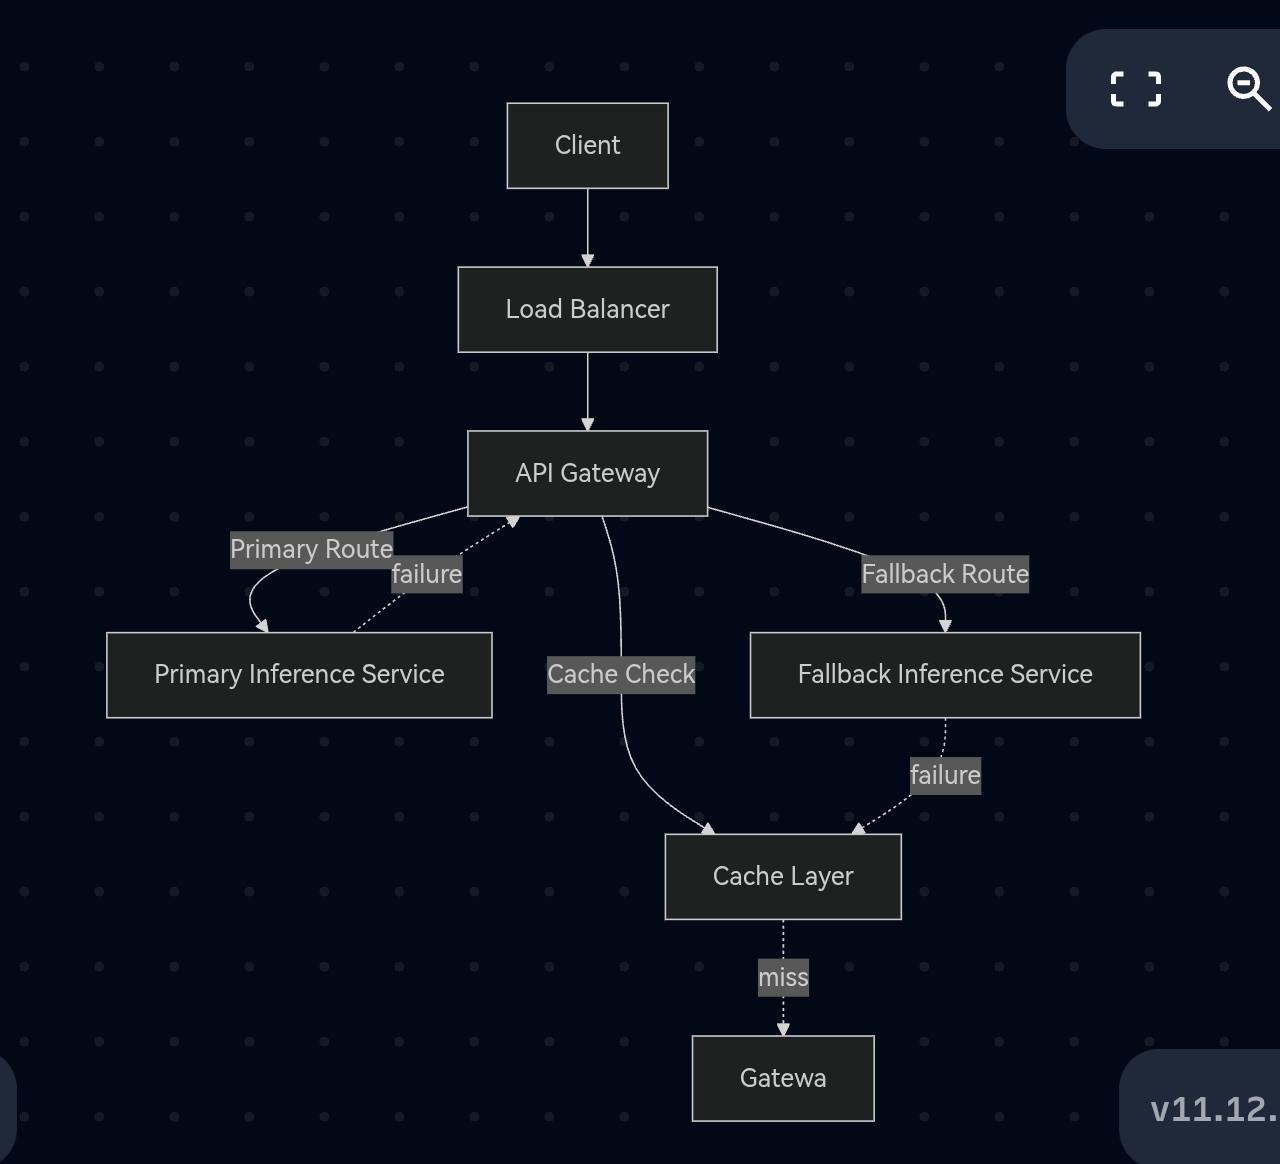
\includegraphics[width=0.9\textwidth]{mermaid.jpg}
\end{center}

\chapter{Conclusion}
Cette architecture modulaire et orientée microservices permet à une plateforme IA de :
\begin{itemize}
    \item Monter en charge (scalabilité horizontale).  
    \item Gérer la tolérance aux pannes (fallback, circuit breaker, cache).  
    \item Garantir sécurité et conformité.  
    \item Exposer des APIs robustes aux développeurs.  
\end{itemize}

\end{document}